\begin{frame}[fragile]{Archive Node}
  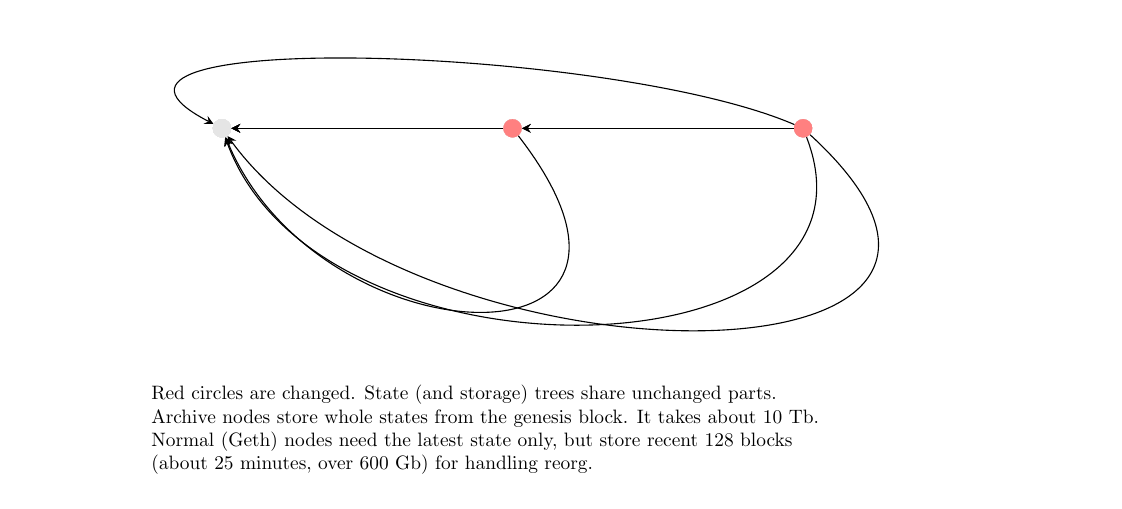
\begin{tikzpicture}[scale=0.7,every node/.style={transform shape}]
  \tikzset{every tree node/.style={align=center}}
  \tikzstyle{n}=[circle,fill,black!10]
  \tikzstyle{changed}=[circle,fill,red!50]

\begin{scope}
\Tree [ % first
  .{block 12345601\\stateRoot}
    [ .\node[n]{};
      [ .\node[n](f3){};
        [ .\node[n]{};
          \node[n]{};
          \node[n]{};
        ]
        [ .\node[n]{};
          \node[n]{};
          \node[n]{};
        ]
      ]
      [ .\node[n]{};
        [ .\node[n]{};
          \node[n]{};
          \node[n](f18){};
        ]
        [ .\node[n]{};
          \node[n]{};
          \node[n](f20){};
        ]
      ]
    ]
    [ .\node[n]{};
      [ .\node[n]{};
        [ .\node[n]{};
          \node[n]{};
          \node[n]{};
        ]
        [ .\node[n]{};
          \node[n]{};
          \node[n](f26){};
        ]
      ]
      [ .\node[n](f6){};
        [ .\node[n]{};
          \node[n]{};
          \node[n]{};
        ]
        [ .\node[n](f14){};
          \node[n]{};
          \node[n]{};
        ]
      ]
    ]
]
\end{scope}

\begin{scope}[xshift=15em]
\Tree [ % second
  .{block 12345602\\stateRoot}
    [ .\node[n](s1){};
      \edge[draw=none] node{}; [ .\node{};
      ]
      [ .\node[n]{};
        [ .\node[n](s9){};
          \node[changed](s19){};
          \edge[draw=none] node{}; \node{};
        ]
        [ .\node[n](s10){};
          \node[changed]{};
          \edge[draw=none] node{}; \node{};
        ]
      ]
    ]
    [ .\node[n](s2){};
      [ .\node[n](s5){};
        [ .\node[n]{};
          \node[changed]{};
          \node[changed]{};
        ]
        [ .\node[n](s12){};
          \node[changed]{};
          \edge[draw=none] node{}; \node{};
        ]
      ]
      \edge[draw=none] node{}; [ .\node{};
      ]
    ]
]
\end{scope}
\draw[-stealth] (s1) -- (f3);
\draw[-stealth] (s9) -- (f18);
\draw[-stealth] (s10) -- (f20);
\draw[-stealth] (s2) -- (f6);
%\draw (s12) -- (f26);
%\draw[-stealth] plot[smooth, tension=0.5] coordinates { (s12) (20em,-25ex) (15em,-28ex) (10em,-28ex) (f26) };
\draw[-stealth] (s12) .. controls (25em,-30ex) and (5em,-28ex) .. (f26);

\begin{scope}[xshift=30em]
\Tree [ % third
  .{block 12345603\\stateRoot}
    [ .\node[n](t1){};
      \edge[draw=none] node{}; [ .\node{};
      ]
      [ .\node[n]{};
        [ .\node[n](t9){};
          \edge[draw=none] node{}; \node{};
          \node[changed]{};
        ]
        [ .\node[n](t10){};
          \node[changed]{};
          \edge[draw=none] node{}; \node{};
        ]
      ]
    ]
    [ .\node[n](t2){};
      \edge[draw=none] node{}; [ .\node{};
      ]
      [ .\node[n](t6){};
        [ .\node[n]{};
          \node[changed]{};
          \node[changed]{};
        ]
        \edge[draw=none] node{}; [ .\node{};
        ]
      ]
    ]
]
\end{scope}
%\draw (t1) -- (f3);
%\draw[-stealth] plot[smooth, tension=0.5] coordinates { (t1) (15em,5ex) (-4em,3ex) (f3) };
\draw[-stealth] (t1) .. controls (20em,10ex) and (-10em,12ex) .. (f3);
\draw[-stealth] (t9) -- (s19);
%\draw (t10) -- (f20);
%\draw[-stealth] plot[smooth, tension=0.5] coordinates { (t10) (30em,-19ex) (16em,-25ex) (5em,-25ex) (f20) };
\draw[-stealth] (t10) .. controls (35em,-30ex) and (5em,-32ex) .. (f20);
\draw[-stealth] (t2) -- (s5);
%\draw (t6) -- (f14);
%\draw[-stealth] plot[smooth, tension=0.5] coordinates { (t6) (35em,-25ex) (13em,-24.5ex) (f14) };
\draw[-stealth] (t6) .. controls (45em,-32ex) and (10em,-32ex) .. (f14);

\node[align=left,anchor=north west] at (-4em,-30ex) {Red circles are changed. State (and storage) trees share unchanged parts.\\
Archive nodes store whole states from the genesis block. It takes about 10 Tb.\\
Normal (Geth) nodes need the latest state only, but store recent 128 blocks\\
(about 25 minutes, over 600 Gb) for handling reorg.};

  \end{tikzpicture}
\end{frame}